\chapter{File Feedrate Control}
\section{Problem Definition}
\hspace*{6mm}Instrument fracture is a potential crisis for endodontic treatment. If a dentist improperly operates an endodontic file, it will increase the possibility of instrument fracture. Most largely, the instrument fracture will happen while a file is inserted into the one-third place far from the root apex. It is barely possible to take out in a small root canal. Removal of broken files is technically tricky, so it is critical to reducing the probability of the instrument fracture.
\par
There is a technical solution to detect a status of a file. When a file suffers a force, it will lead to the crystalline phase transformation. However, it can only be observed from a microscope. It is impracticable to usually monitor it during the surgery. Previous literature shows there are two main causes of fractured files are torsional fracture and flexural fatigue, which account for 55.7\% and 44.3\% separately\cite{SATTAPAN2000161}. Therefore, we can reduce the torque a file bears to prevent the instrument fracture.
\section{The Proposed Method and Theorem}
\hspace*{6mm}In order to protect an endodontic file from fracturing, we need to reduce the file torque. The easiest and most effective way to solve this issue would be monitoring the torque which the file is enduring. Therefore, we implement a torque monitoring system on DentiBot. We utilize current feedback to keep track of the torque. An increase in the current of the motor is indicative of the contact resistance of the file. Also, We propose two approaches both based on feedrate control to release the file torque. One is inverse rotation control discussed in section \ref{sec:Inver Rotation Control}and the other is feed control discussed in section \ref{sec:Feed Control}, they are both efficient ways to release the file torque. Once the current of the file is in excess of a threshold, it will inversely rotate or decline the feedrate to release torque. 
\subsubsection{Theorem}
\hspace*{6mm}A motor can be modeled as an RL circuit. In this way, we can get the following formula 
\begin{equation}
\begin{split}
V = R \cdot I + L  \cdot \frac{\mathrm{d}I}{\mathrm{d}t} + \varepsilon
\end{split}
\end{equation}
where $V$ represents the input voltage, $I$ represents the input current, and $\varepsilon $ represents the back EMF produced by the motor motion.
\par
Since the value of the inductance of DC motor is small, we ignore the inductance term L. After transposition, we can get the following relation between the current and the back EMF.
\begin{equation}
\label{eq:current and the back EMF}
\begin{split}
I = \frac{I - \varepsilon}{R}
\end{split}
\end{equation}
\par\noindent
The back EMF produced by the motor is dependent upon the motor constant $K$, shown as the following equation.
\begin{equation}
\label{eq: the back EMF}
\begin{split}
\varepsilon  = K \cdot \frac{\mathrm{d}\theta (t)}{\mathrm{d}t} = K \cdot \omega (t)
\end{split}
\end{equation}
\par
When the file encounters resistance during the drilling procedure, the rotating speed of the motor would slow down. With the Equation \ref{eq:current and the back EMF} and \ref{eq: the back EMF} we can infer that the back EMF would decrease, and the current would increase.
Also, we have the relation between the current and torque
\begin{equation}
\begin{split}
T_m = K_m  \cdot \ I
\end{split}
\end{equation}
where $k_m$ represent the torque constant of a motor.
\par\noindent
The maximum torque a root canal file can bear is $6.20$ Ncm ($62.0$ mNm) \cite{boessler2009effect}. Therefore, we can derive the following inequality.
\begin{equation}
\begin{split}
T_m \cdot \mathrm{GR} < 62 \text{ (mNm)}
\end{split}
\end{equation}
where $\mathrm{GR}$ is gear ratio of gearbox mounted on a motor.
\par
Hence, we can set a current threshold based on the following condition. 
\begin{equation}
\begin{split}
I_{max} < \frac{62}{\mathrm{GR} \cdot K_m}
\end{split}
\end{equation} 
In reality, $\mathrm{GR}$ is $67$ and $K_m$ is $16 \text{mNm/A}$
\subsection{Feedrate Control - Inverse Rotation Control}
\label{sec:Inver Rotation Control}
\hspace*{6mm}Once the current of the file exceeds the specific threshold, it will inversely rotate for 90 degrees to release torque and then continue drilling in the original direction. Before designing the DentiBot, we have validated this function with the prototype of DentiBot shown as Fig \ref{fig: prototype}.
\begin{figure}[htbp]
\begin{center}
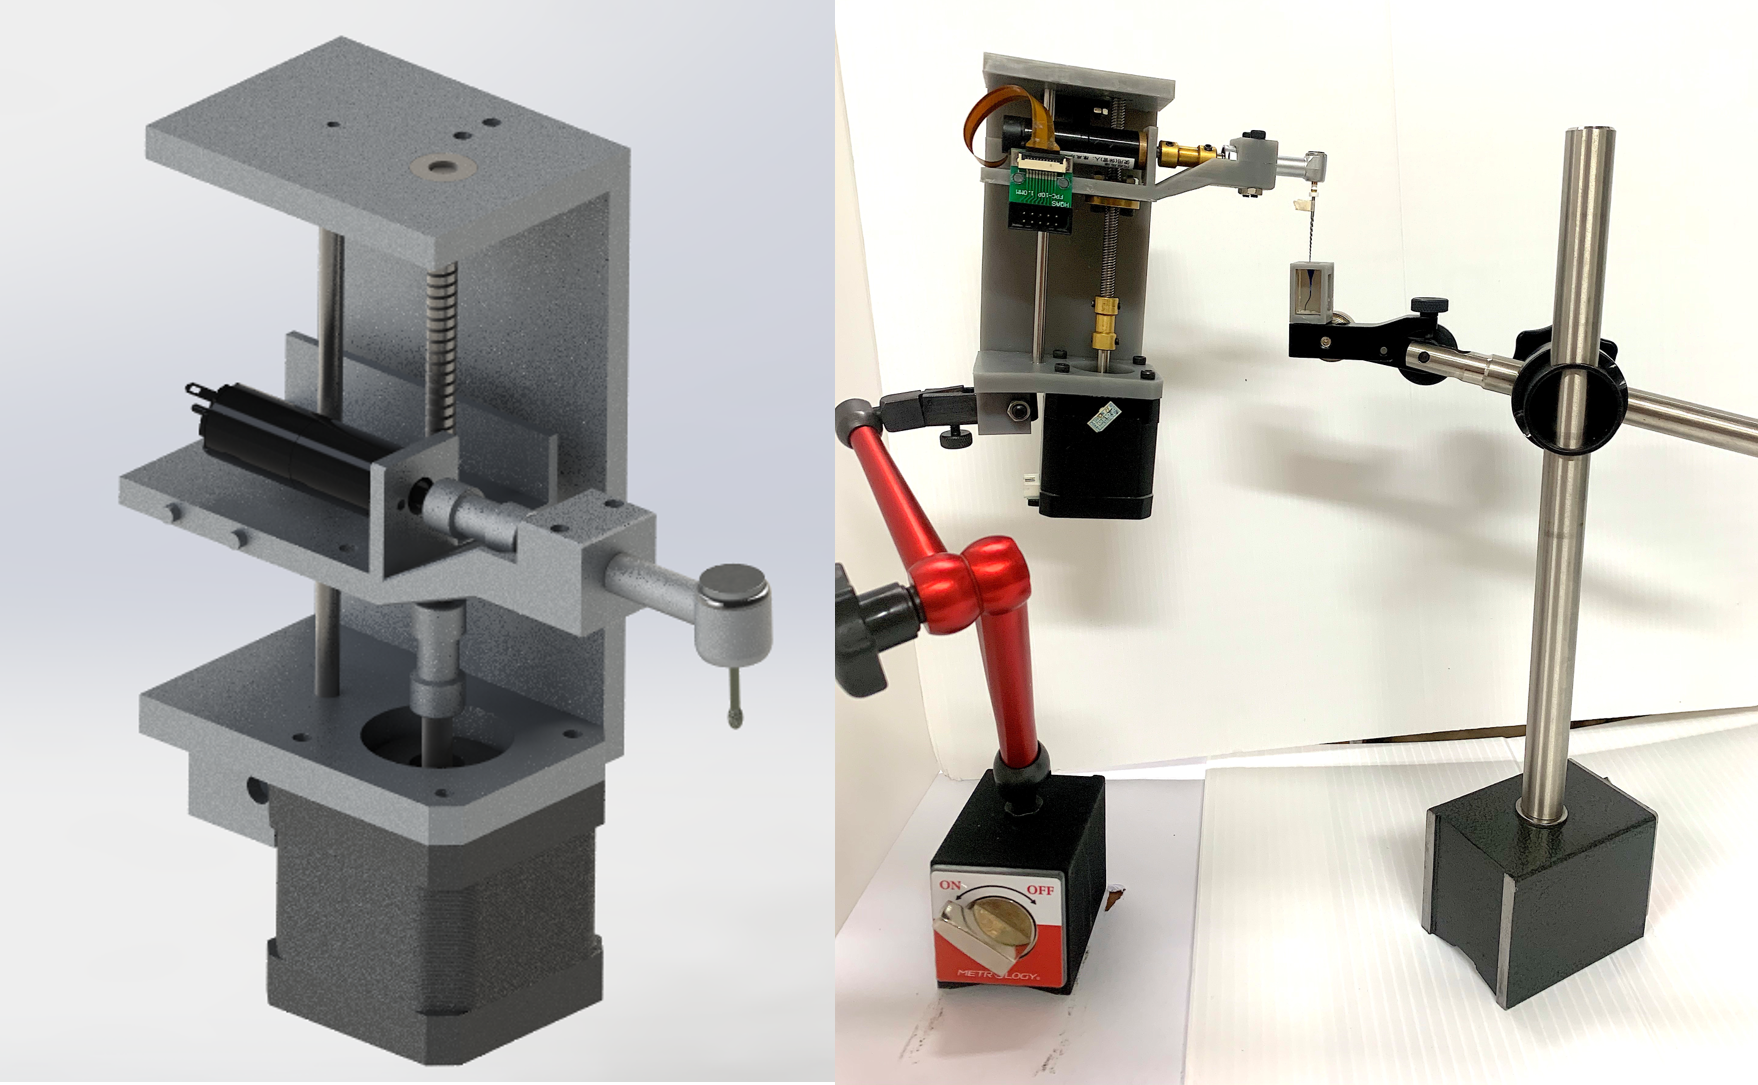
\includegraphics[width=1\linewidth]{Images/Prototype.png}
\caption{The prototype of DentiBot
}\label{fig: prototype}
\end{center}
\end{figure}	
\par
It is a drilling system mounted on a magnetic stand. The modified handpiece, a hand-held dental electric device, with a single axis mechanism can validate the inverse rotation control. 
\begin{figure}[htbp]
\begin{center}
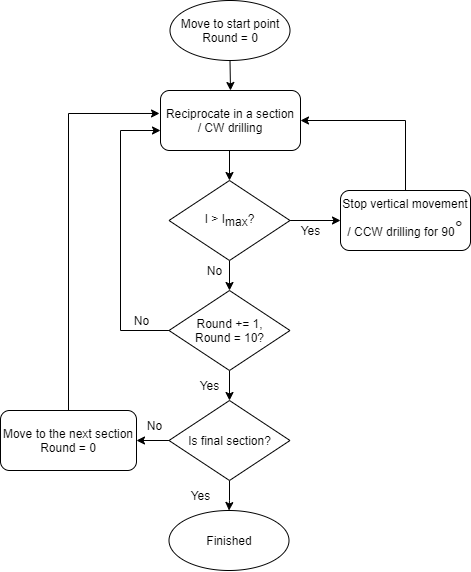
\includegraphics[width=0.8\linewidth]{Images/inverse_rotation.png}
\caption{Motion planning of Inverse Rotation Control.}
}\label{fig: inverse_rotation}
\end{center}
\end{figure}
\par
We designed motion planning to perform the drilling procedure. The root canal is divided into several sections. In Fig \ref{fig: inverse_rotation}, we propose a motion planning to validate the function.In the beginning, the robot moves to the start point and then repetitively drills one section back and forth at least ten times until the current feedback decrease under the specific threshold. If the current exceeds the threshold, the endodontic file will inversely rotate for $90^o$ to release the torque and then drill the same section again. After one section is cleaned thoroughly, the drilling file will move to the next section. Every section will be cleaned for at least $10$ rounds. If there is reverse rotation, it will be more than $10$ rounds. When to be finished is contingent on whether the endodontic file reaches the final section.
\subsection{Feedrate Control - Feed Control}
\label{sec:Feed Control}
\hspace*{6mm}As mentioned above, we can detect the current to estimate the torque and inversely rotate the motor if the current exceeds the threshold current. However, inverse rotation control is just mimicking a dentist to perform endodontic treatment. Time-consuming is still a problem. Therefore, we propose the other method to improve this problem. Previous literature which dedicate to a form drilling with torque control is similar to our root drilling \cite{boessler2009effect}. We propose a similar control scheme for our root drilling.
\begin{figure}[htbp]
\begin{center}
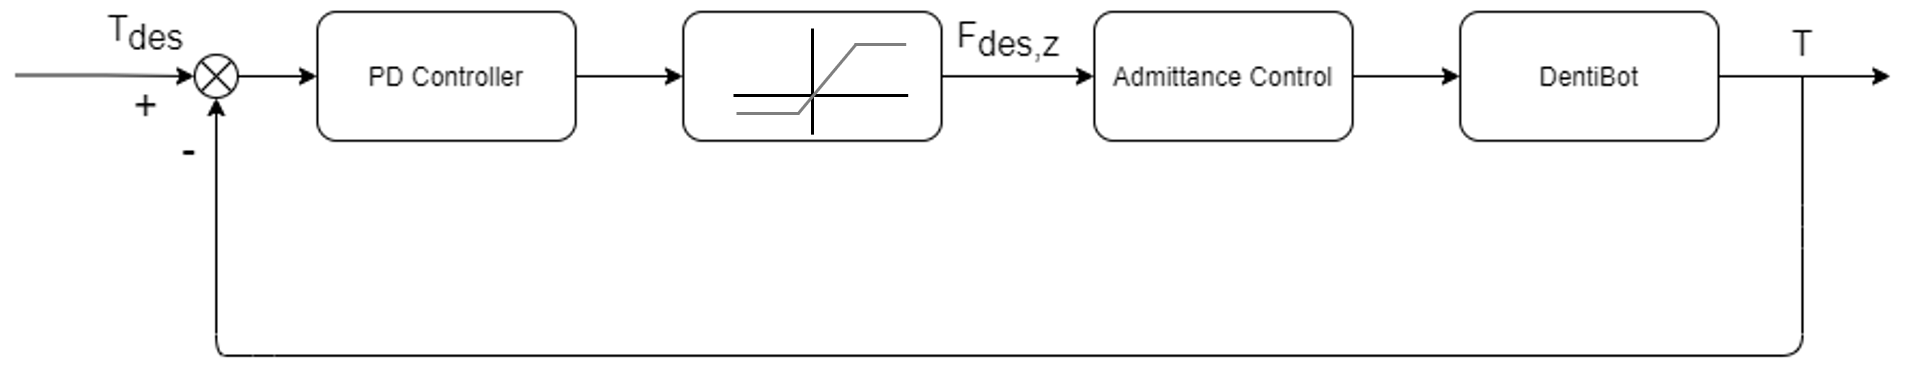
\includegraphics[width=1\linewidth]{Images/feedrate_control.png}
\caption{Control scheme of Feedrate Control.}
}\label{fig: feed_control}
\end{center}
\end{figure}
\par
To put it simply, we regulate the feedrate to control the torque the file bears.


\begin{figure}[htbp]
\begin{center}
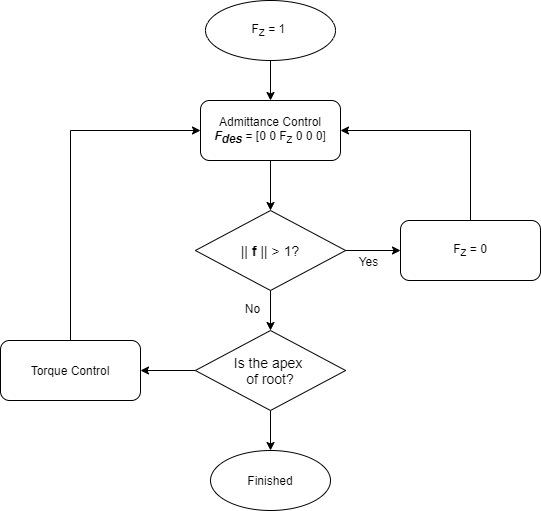
\includegraphics[width=0.8\linewidth]{Images/torque_control.png}
\caption{Flow chart of Feed Control. $f$ represents force vector}
}\label{fig: feed_control}
\end{center}
\end{figure}